\section{3. General vector spaces}
% *********************************

\subsection{Linear systems revisted}
% ==================================

It is useful to keep in mind that all these statements are equivalent. If one is
true all the others are true. Given a $n$ by $n$ (square) matrix \textbf{A} we have:

\begin{itemize}
\item \textbf{A} is invertible.
\item \textbf{A} is full rank, \emph{i.e.} $rank(\mathbf{A}) = nrows(\mathbf{A}) = n$.
\item Rows in \textbf{A} are linearly independent.
\item Columns in \textbf{A} are linearly independent.
\item $nullity(\mathbf{A}) = 0$.
\item The \emph{nullspace} of \textbf{A} contains only the zero vector.
\end{itemize}

Given the system $\mathbf{Ax = O}$, the \textbf{\emph{nullspace}} is the set of
vectors that satisfies the system. The \emph{dimension} of the nullspace is called
\textbf{\emph{nullity}}. Consequently for a $n$ by $n$ matrix we have:

$$
rank(\mathbf{A}) + nullspace(\mathbf{A}) = n
$$

\subsubsection{Exercise 3.6.1}
%-----------------------------

Nullspace of 2 by 2 unit matrix $\left[\begin{matrix}1 & 0\\0 & 1\end{matrix}\right]$
is the zero vector since this is the only solution to $\mathbf{Av = O}$.

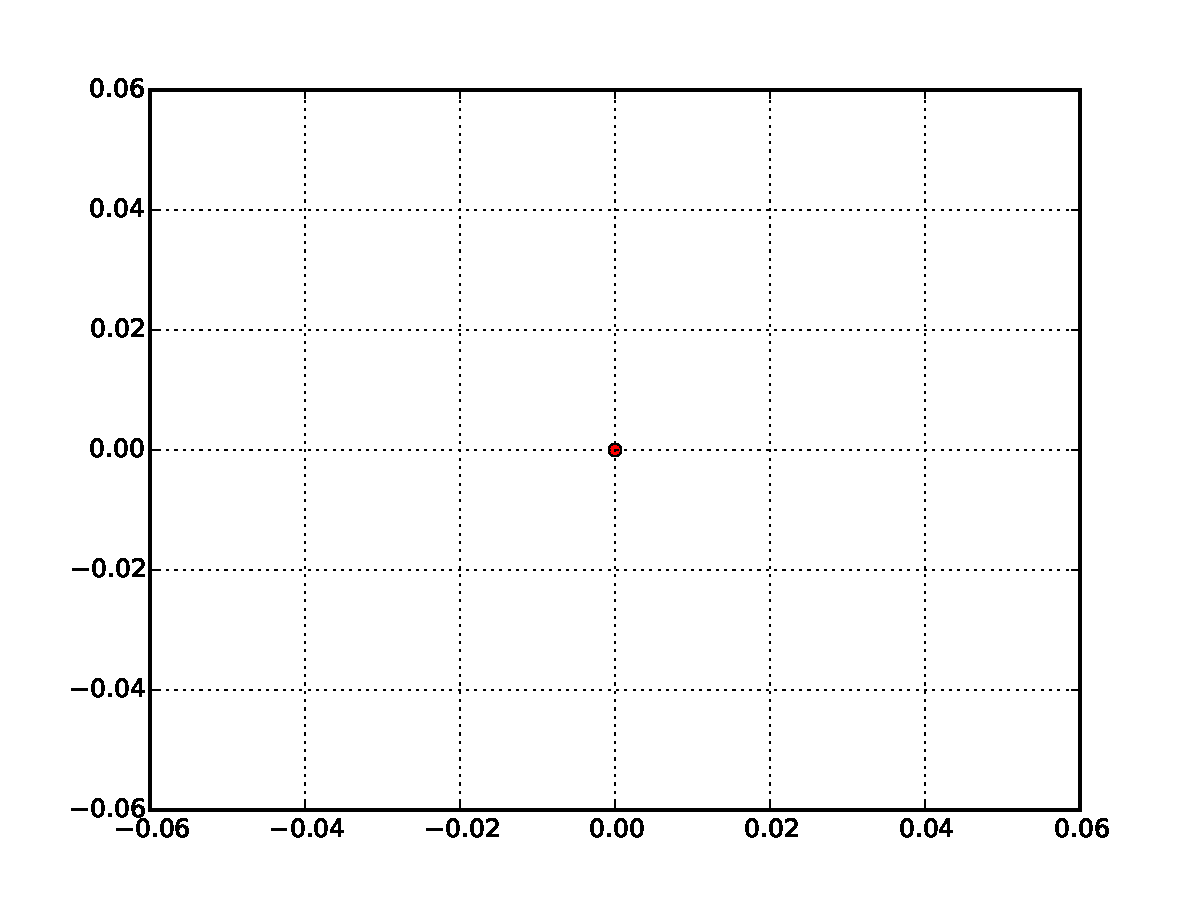
\includegraphics[width=0.7\linewidth]{figs/ex3_6_1.pdf}

\begin{verbatim}
x,y= symbols('x,y')
v= Matrix([x, y])
A= eye(2)

sols= solve(Eq(A*v, Matrix([0, 0])))[0] ## [{x: 0, y: 0}]
A.nullpsace() ## Empty. 

plt.plot(sols[x], sols[y], 'ro')
plt.grid()
plt.savefig('figs/ex3_6_1.pdf')
\end{verbatim}

For $\mathbf{A}= \left[\begin{matrix}1 & 2\\2 & 4\end{matrix}\right]$ we need to
solve $\left[\begin{matrix}x + 2 y\\2 x + 4 y\end{matrix}\right] = \left[\begin{matrix}0\\0\end{matrix}\right]$.
Solution is $\left \{ x : - 2 y\right \}$ or $\left[\begin{matrix}-2\\1\end{matrix}\right]$.
Graphically, the nullspace is the vector passing by $\left[\begin{matrix}-2\\1\end{matrix}\right]$
as shown here below. In fact any point sitting on this line will make $\mathbf{Av = O}$.
\emph{E.g.} with $\mathbf{v} = [2\ -1]^T$ we have $\left[\begin{matrix}1 & 2\\2 & 4\end{matrix}\right] \left[\begin{matrix}2\\-1\end{matrix}\right] =
\left[\begin{matrix}0\\0\end{matrix}\right]$

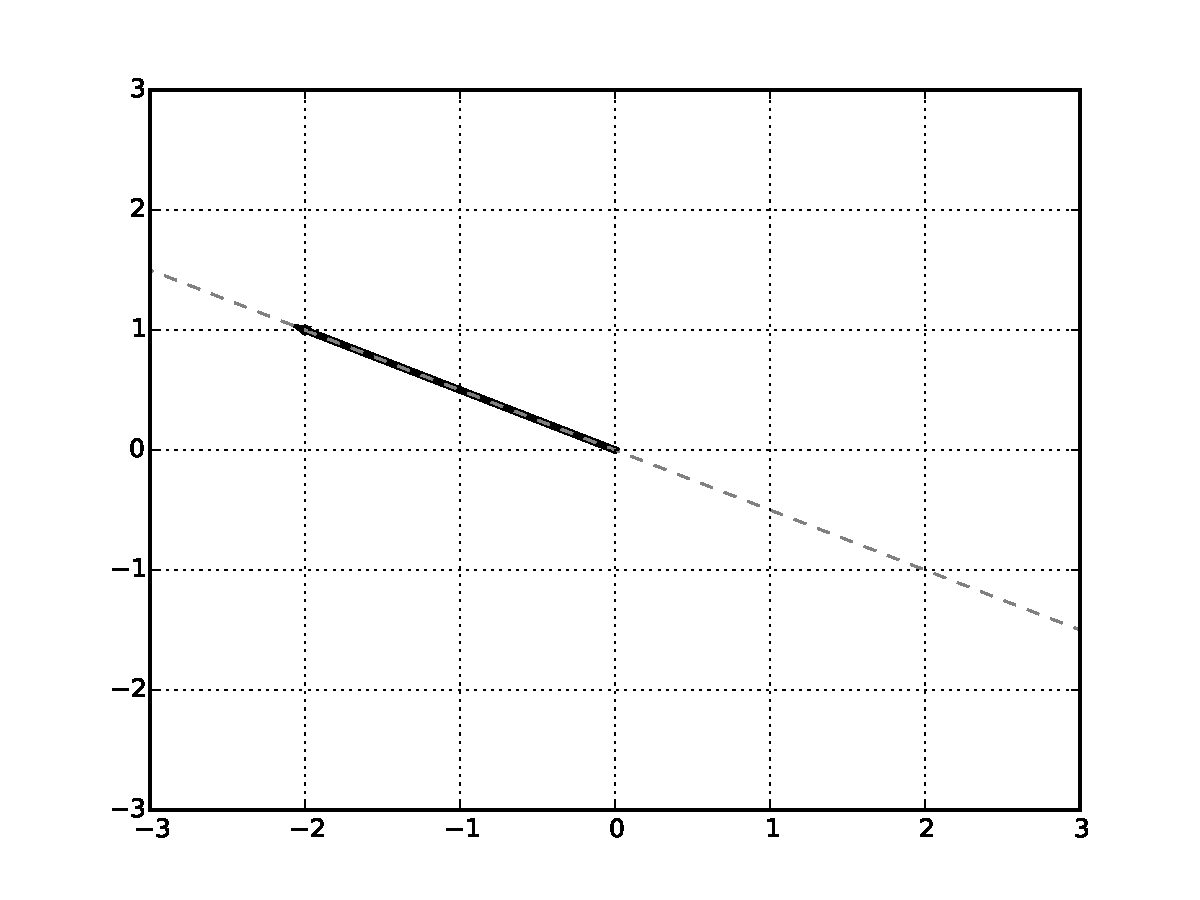
\includegraphics[width=0.7\linewidth]{figs/ex3_6_1b.pdf}

\begin{verbatim}
A= Matrix(2, 2, [1, 2, 2, 4])

sols= solve(Eq(A*v, zeros(A.rows, 1)))[0]
## Or simply
nsp= A.nullspace()[0]

plt.plot((0, nsp[0]*3), (0, nsp[1]*3))

plt.plot((-nsp[0]*3, nsp[0]*3), (-nsp[1]*3, nsp[1]*3), color= 'grey',
    linestyle= '--')
plt.arrow(0, 0, float(nsp[0]), float(nsp[1]), 'g', lw= 3)
plt.xlim(-3, 3)
plt.ylim(-3, 3)
plt.grid()
plt.savefig('figs/ex3_6_1b.pdf')
\end{verbatim}

For $\left[\begin{matrix}1 & 0\\1 & 2\\6 & 10\end{matrix}\right]$ we need to solve
$\left[\begin{matrix}x\\x + 2 y\\6 x + 10 y\end{matrix}\right] = \left[\begin{matrix}0\\0\\0\end{matrix}\right]$.
This is for $\left \{ x : 0, \quad y : 0\right \}$.

\begin{verbatim}
A= Matrix(3, 2, [1, 0, 1, 2, 6, 10])

sols= solve(Eq(A*v, zeros(A.rows, 1)))[0]
## Or
A.nullspace() # -> []
\end{verbatim}


For $\left[\begin{matrix}1 & 2\\3 & 4\\5 & 6\end{matrix}\right]$ we have
$\left[\begin{matrix}x + 2 y\\3 x + 4 y\\5 x + 6 y\end{matrix}\right] = \left[\begin{matrix}0\\0\\0\end{matrix}\right]$
solved only for $x= 0; y= 0$

\begin{verbatim}
A= Matrix(3, 2, [1, 2, 3, 4, 5, 6])
sols= solve(Eq(A*v, zeros(A.rows, 1)))[0]
\end{verbatim}

\subsubsection{Exercise 3.6.3}
%-----------------------------
Determine nullspace and nullity for
$\mathbf{A} = \left[\begin{matrix}1 & -2 & -3\\4 & -5 & -6\\7 & -8 & -9\end{matrix}\right]$.

The solution to 
$\left[\begin{matrix}x - 2 y - 3 z\\4 x - 5 y - 6 z\\7 x - 8 y - 9 z\end{matrix}\right] =
\left[\begin{matrix}0\\0\\0\end{matrix}\right]$.

is $\left \{ x : - z, \quad y : - 2 z\right \}$. Rearranged in vector form we have
$\left[\begin{matrix}x\\y\\z\end{matrix}\right] =
\left[\begin{matrix}-z\\-2z\\z\end{matrix}\right] =
z(\left[\begin{matrix}-1\\-2\\1\end{matrix}\right])
$ for $z$ being any real. Note therefore that the nullspace is the solution to the
linear system.

The nullity is the dimension of the nullspace. In this case only one vector makes
the nullspace, hence $nullity(\mathbf{A}) = 1$

\begin{verbatim}
A= Matrix([[1, -2, -3],
           [4, -5, -6],
           [7, -8, -9]])
x,y,z= symbols('x,y,z')
v= Matrix([x, y, z])
sols= solve(Eq(A*v, zeros(A.rows, 1)), x)[0]
v.subs(sols)
# Also
nsp= A.nullspace() # -> [[-1, -2, 1]]
nlty= len(nsp)     # -> 1
\end{verbatim}

For $\mathbf{A} = \left[\begin{matrix}2 & -2 & -2\\4 & -4 & -4\\8 & -8 & -8\end{matrix}\right]$
the linear systen to solve is
$\left[\begin{matrix}2 x - 2 y - 2 z\\4 x - 4 y - 4 z\\8 x - 8 y - 8 z\end{matrix}\right] =
\left[\begin{matrix}0\\0\\0\end{matrix}\right]$. Solved for $\left \{ x : y + z\right \}$.
Substituing the results in \textbf{v} we have the nullspace:

$
\mathbf{v_{sol}} = \left[\begin{matrix}x\\y\\z\end{matrix}\right] =
\left[\begin{matrix}y + z\\y\\z\end{matrix}\right] =
y(\left[\begin{matrix}1\\1\\0\end{matrix}\right]) + z(\left[\begin{matrix}1\\0\\1\end{matrix}\right])
$

The nullspace is made of two vectors $y(\left[\begin{matrix}1\\1\\0\end{matrix}\right]) + z(\left[\begin{matrix}1\\0\\1\end{matrix}\right])$
hence the nullity is 2. Note that $rank(\mathbf{A}) = 1$ consistent with $nullity(\mathbf{A}) + rank(\mathbf{A}) = n$

\begin{verbatim}
A= Matrix([[2, -2, -2],
           [4, -4, -4],
           [8, -8, -8]])
sols= solve(Eq(A*v, zeros(A.rows, 1)), x)
v.subs(sols)
# Equivalent to
y*Matrix([1,1,0]) + z*Matrix([1, 0, 1])
# Same as
nsp= A.nullspace()
nlty= len(nsp)
\end{verbatim}

This system
$\left[\begin{matrix}2 x + 9 y - 3 z\\5 x + 6 y - z\\9 x + 8 y - 9 z\end{matrix}\right] =
\left[\begin{matrix}0\\0\\0\end{matrix}\right]$
has solution only for $\left [ \left \{ x : 0, \quad y : 0, \quad z : 0\right \}\right ]$
hence the nullspace is the zero vector and the nullity is 0. In fact, the
dimension of the zero vector is zero.

\begin{verbatim}
A= Matrix([[2, 9, -3],
           [5, 6, -1],
           [9, 8, -9]])
sols= solve(Eq(A*v, zeros(A.rows, 1)))
nsp= A.nullspace() # -> []
nlty= len(nsp)     # -> 0
\end{verbatim}

Same as above for $\mathbf{A}= \left[\begin{matrix}-3 & 1 & -1\\2 & 5 & -7\\4 & 8 & -4\end{matrix}\right]$

\begin{verbatim}
A= Matrix([[-3, 1, -1],
           [2, 5, -7],
           [4, 8, -4]])
sols= solve(Eq(A*v, zeros(A.rows, 1)))
\end{verbatim}

\subsubsection{Exercise 3.6.4}
%-----------------------------

Determine the nullspace and nullity of
$\left[\begin{matrix}1 & 2 & 3 & 4 & 5 & 6 & 7\\
                     8 & 9 & 10 & 11 & 12 & 13 & 14\\
                     15 & 16 & 17 & 18 & 19 & 20 & 21\\
                     22 & 23 & 24 & 25 & 26 & 27 & 28\\
                     29 & 30 & 31 & 32 & 33 & 34 & 35\end{matrix}\right]$

Nullspace is
$
\left [ \left[\begin{matrix}1\\-2\\1\\0\\0\\0\\0\end{matrix}\right], \quad
        \left[\begin{matrix}2\\-3\\0\\1\\0\\0\\0\end{matrix}\right], \quad
        \left[\begin{matrix}3\\-4\\0\\0\\1\\0\\0\end{matrix}\right], \quad
        \left[\begin{matrix}4\\-5\\0\\0\\0\\1\\0\end{matrix}\right], \quad
        \left[\begin{matrix}5\\-6\\0\\0\\0\\0\\1\end{matrix}\right]\right ]
$ contaning five vectors, five is the nullity of \textbf{A}.

\begin{verbatim}
x1,x2,x3,x4,x5,x6,x7= symbols('x1:8')
A= Matrix(5, 7, range(1, 36))
sols= solve(Eq(A*v, zeros(A.rows, 1)))
v.subs(sols) # Nullspace. You could read out the nullspace vectors from here
nsp= A.nullspace()
nly= len(A) # 5
\end{verbatim}

\subsubsection{Exercise 3.6.5}
%-----------------------------

Determine bases for row, column and null space for
$\mathbf{A} = \left[\begin{matrix}1 & -4 & -9\\2 & 5 & -7\end{matrix}\right]$.

In other words, we need to find a set of \textbf{linearly independent} vectors such that
every vector in the given vector space (e.g. row space) is \textbf{linearly dependent} of these
vectors. Bases or coordinates are the basic building blocks to represent a vector
space.

To find a basis for the rows of a matrix (i.e. for this vector space) we need to
put the matrix un RREF. The rows of the RREF matrix are linearly independent. For
the rows in \textbf{A},
$\mathbf{A_{rref}} =
\left[\begin{matrix}1 & 0 & - \frac{73}{13}\\0 & 1 & \frac{11}{13}\end{matrix}\right] =
\left[\begin{matrix}13 & 0 & -73\\0 & 13 & 11\end{matrix}\right]$,

the rows of $\mathbf{A_{rref}}$ are the bases for the row space of $\mathbf{A}$.

The basis for the column vector can be obtained by looking at the leading 1s in
$A_{rref}$, these are $\left[\begin{matrix}1 & 0\\0 & 1\end{matrix}\right]$. \emph{
The same conclusion is reached by transposing \textbf{A} and repeating the reasoning
for the row space. Like \texttt{A.transpose().rref()}}

The basis for the nullspace is given by a nullspace itself \texttt{A.nullspace()}
which is $\left[\begin{matrix}\frac{73}{13}\\- \frac{11}{13}\\1\end{matrix}\right]$.
In this case the nullity is 1.

\begin{verbatim}
A= Matrix(2, 3, [1, -4, -9, 2, 5, -7])
B= Matrix(3, 2, [1, 3, 2, 5, -14, -37])
C= Matrix([[1, 3, -9, 5],
           [2, 6, 7, 1],
           [1, 3, -8, 1]])
rbasis= rref= A.rref()
cbasis= rref.A.transpose().rref()
nspbasis= A.nullspace()
\end{verbatim}